\documentclass[xodstep]{wnspt}

\author      {Grzegorz Gromko}
\nralbumu    {80385}
\kierunek    {Informatyka}
\specjalnosc {Inżynieria oprogramowania}
\date        {2024}
\miejsce     {Częstochowa,}
\opiekun     {dr hab. Andrzej Zbrzezny, prof. UJD}
\opiekunpom  {}

\usepackage{amsmath}
\usepackage{amsfonts}
\usepackage{amsthm}
\usepackage{amssymb}
\usepackage[T1]{fontenc}
\usepackage[utf8]{inputenc}
\usepackage[polish]{babel}
\usepackage{polski}
\usepackage{times}
\usepackage{colortbl}
\usepackage{hyperref}
\usepackage{multibib}
\usepackage{url}
\usepackage{setspace}
\usepackage{indentfirst}
\usepackage{listingsutf8}
\usepackage{beramono}
\usepackage[section]{placeins}
\usepackage{csquotes}
\usepackage{abstract}
%\usepackage[%backend=biber,refsegment=section,defernumbers=true,]{biblatex}

\lstset { %
language=csh,                  % choose the language of the code
basicstyle=\ttfamily,           % the fonts that are used for the code
numbers=left,                   % where to put the line-numbers
numberstyle=\footnotesize,      % the size of the fonts that are used for the line-numbers
stepnumber=1,                   % the step between two line-numbers. If it's 1 each line will be
numbersep=5pt,                  % how far the line-numbers are from the code
showspaces=false,               % show spaces adding particular underscores
showstringspaces=false,         % underline spaces within strings
showtabs=false,                 % show tabs within strings adding particular underscores
frame=single,                   % adds a frame around the code
tabsize=4,                      % sets default tabsize to 2 spaces
captionpos=b,                   % sets the caption-position to bottom
breaklines=true,                % sets automatic line breaking
breakatwhitespace=false,        % sets if automatic breaks should only happen at whitespace
escapeinside={\%*}{*)}         % if you want to add a comment within your code 
}

\newcommand{\R}{mathbb{R}}

\renewcommand{\lstlistlistingname}{Spis listingów}
\renewcommand{\lstlistingname}{Listing}

\newtheorem{lemat}{Lemat}
\newtheorem{twierdzenie}{Twierdzenie}

\title{ Projekt i implementacja programu do optycznego rozpoznawania i przetwarzania zapisu nutowego do formatu MIDI w języku Python
\\{~}
Design and implementation of a program for optical recognition and processing of musical notation to MIDI format in Python}

\frenchspacing

\begin{document}

\maketitle
\onehalfspacing

\begin{abstract}
	Celem niniejszej pracy jest stworzenie programu służącego do optycznego rozpoznawania zapisu nutowego z plików graficznych oraz przetworzenia wydobytych informacji semantycznych do pliku w formacie MIDI. Program posiada system automatycznego usuwania wypaczania obrazu, a także możliwość utworzenia pliku graficznego z uzyskanych danych, pozwalając na digitalizację zapisu nutowego.
\end{abstract}



\introduction

Tu wprowadzenie w tematykę, motywacja, cel pracy, układ rozdziałów.

\chapter{Specyfikacja wymagań}
W tym rozdziale zawarto wymagania postawione programowi przeznaczonemu do odczytywania notacji muzycznej z plików graficznych oraz konwersją odczytanych danych do formatu MIDI.

\section{Wymagania biznesowe}
Nazwa programu to "Photo-2-MIDI". Przeznaczeniem oprogramowania jest umożliwienie użytkownikom zdigitalizowanie w przystępny sposób drukowanych zapisów nutowych ze zdjęć lub skanów do plików MIDI.

\section{Słownik skrótów i pojęć}

	\begin{enumerate}
		\item Notacja muzyczna, pismo nutowe, zapis nutowy - symboliczny język reprezentujący odbieraną słuchowo muzykę graną na instrumentach, czy też śpiewaną przez ludzki głos, przy pomocy symboli reprezentujących dźwięki, ich długość oraz wysokość, jak i brak tych dźwięków używając znaków pauz. Przy pomocy takiego języka można zapisać niemal wszystkie cechy dźwięków, takie jak rytmika, melodia, harmonia, dynamika czy artykulacja. W tej pracy pojęcia te będą odnosić się do nowożytnej zachodniej notacji muzycznej.
		
		\begin{figure}
			\centering
			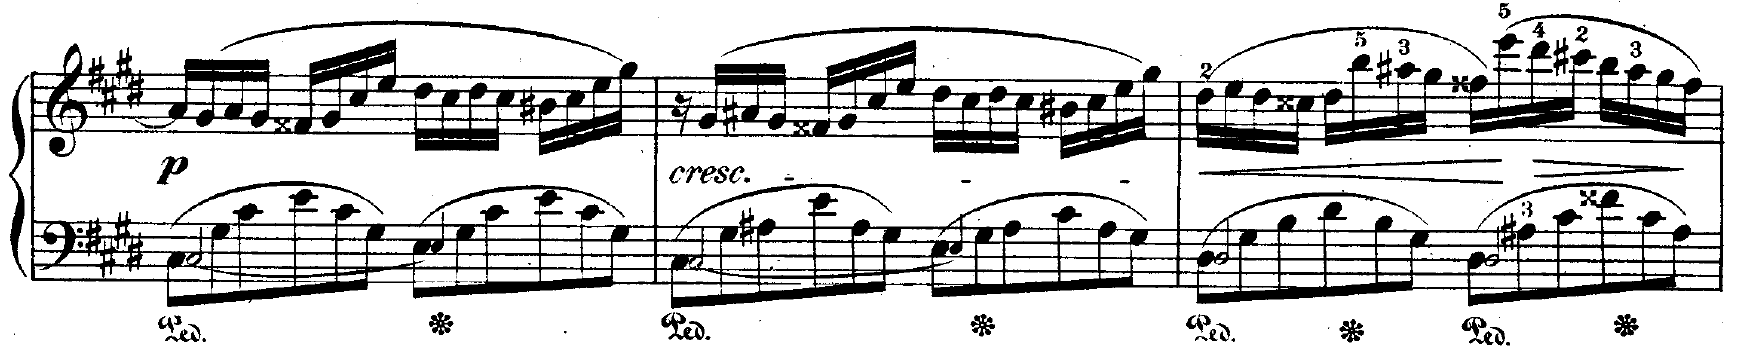
\includegraphics[width=14cm]{images/chopin_fastasie_impromtu_no_4_op_66.png}
			\caption{Fragment \textit{Fantasie-Impromptu cis-moll op. 66} Fryderyka Chopina zapisany w nowożytnej zachodniej notacji muzycznej. }
			\label{fig:chopin_impromptu}
		\end{figure}
		
		\item format MIDI - (ang. Musical Instrument Digital Interface) popularny format plików, który w przeciwieństwie do standardowych formatów audio nie przenosi bezpośrednich informacji o dźwięku, tylko informacje o granych nutach, ich synchronizacji, trwaniu oraz głośności. 
	\end{enumerate}

\section{Wymagania funkcjonalne}
	\begin{enumerate}
		\item Użytkownik może wprowadzić plik lub pliki zawierające drukowane pismo nutowe w standardowej zachodniej notacji nutowej w formatach PNG, JPG, PDF.
		\item Użytkownik może wygenerować na podstawie wprowadzonych plików pojedynczy plik MIDI.
		\item Użytkownik może wygenerować na podstawie wprowadzonych plików oddzielne pliki MIDI dla każdego pliku.
	\end{enumerate}
	
	
\section{Wymagania niefunkcjonalne}
Program wymaga do działania:
	\begin{enumerate}
		\item Języka Python w wersji 3.11
	\end{enumerate}
\chapter{Technologie wykorzystane w projekcie}

W drugim rozdziale przedstawiono technologie wykorzystane w implementacji programu. Głównymi czynnikami wyboru danych technologii była łatwość użycia oraz ich możliwości.

Najważniejszymi punktami wybranych technologii są m.in.:
\begin{itemize}
	\item Otwarty kod źródłowy
	\item Popularność
	\item Ogólnodostępność
	\item Aktywna społeczność rozwijająca projekty
	\item Łatwość wykorzystania
	\item Dostępności informacji dot. technologii
\end{itemize}

Dzięki powyższym cechom wykazywanym przez użyte technologie mamy zapewnioną szybkość tworzenia oprogramowania, gdzie w przypadku napotkania błędów w procesie jego kreacji możemy liczyć na pomoc społeczności w jego rozwiązaniu jak i szeroką gamę wcześniej stworzonych narzędzi.



\section{Python 3}
Sercem każdego programu jest język, w którym został on napisany. Językiem programowania, wybranym do implementacji projektu jest \textbf{Python} w wersji 3.11.
Jest to wysokopoziomowy, wieloparadygmatowy język skryptowy ogólnego przeznaczenia, którego ideą przewodnią jest czytelność uzyskanego kodu źródłowego. Powstał w 1991 roku i jest ciągle rozwijany oraz cieszy się od wielu lat niesłabnącą popularnością, która wynika między innymi z:

\begin{itemize}
	\item Łatwość nauki
	\item Dostępności materiałów dydaktycznych
	\item Wszechstronności języka
	\item Mnogości różnorodnych bibliotek
	\item Wieloplatformowość
\end{itemize}

\section{PyTorch}
Otwartoźródłowa biblioteka uczenia maszynowego stworzona przez Facebook AI Research (teraz Meta AI), bazowana na Pythonie i Torch-u, głównie używana do aplikacji uczenia maszynowego używających procesorów graficznych i TPU. PyTorch jest preferowany przez wielu badaczy sztucznej inteligencji przez używanie dynamicznych grafów obliczeń, co pozwala na uruchamianie i testowanie małych części kodu w czasie rzeczywistym bez potrzeby implementacji całości kodu, móc sprawdzić czy dana część kodu działa czy nie.

Głównymi zaletami PyTorch są:
\begin{itemize}
	\item Obliczenia tensorowe z dobrym wsparciem przyśpieszenia sprzętowego GPU i TPU
	\item Automatyczne różnicowanie dla tworzenia i trenowania głębokich sieci neuronowych
\end{itemize}

\section{OpenCV}
OpenCV (Open Source Computer Vision Library) jest otwartoźródłową biblioteką widzenia maszynowego oraz uczenia maszynowego. Została ona zbudowana by dostarczyć wspólną infrastrukturę dla aplikacji rozpoznawania obrazów oraz przyśpieszenia użycia percepcji maszynowej w produktach komercyjnych.

\section{Pillow}
Biblioteka będąca odgałęzieniem Python Imaging Library (PIL), która to dodaje możliwości przetwarzania obrazów do programów pisanych w języku Python. Dodaje ona szerokie wsparcie formatów plików, wydajną wewnętrzną reprezentację oraz duże możliwości przetwarzania obrazów. 

\section{Verovio Toolkit}
Verovio jest szybką, przenośną i lekką biblioteką do grawerowania cyfrowych zapisów nutowych MEI (Musical Encoding Initiative) do obrazów formatu SVG. Zawiera również konwertery do renderowania cyfrowych zapisów nutowych formatów MusicXML, Musedata, EsAC czy Humdrum.
\chapter{Budowa programu}
W rozdziale trzecim zawarto informacje dotyczące budowy programu. Na początku opisana jest jego struktura w postaci diagramów. Następnie opisane są poszczególne fragmenty programu. Na końcu znajduje się opis interfejsu graficznego programu.


\section{Struktura programu}

Poniżej znajduje się opis struktury plików oraz opis zawartości poszczególnych katalogów programu.

\begin{itemize}
	\item \textbf{photo-2-midi.py} - interfejs programu, uruchamia program.
	\item \textbf{convert\_to\_MIDI.py} - główna część programu, zarządza działaniem procesu uzyskiwania informacji ze zdjęć.
	\item \textbf{staff\_detection.py} - w skład tego pliku wchodzą funkcje odpowiedzialne za detekcję pięciolinii.
	\item \textbf{dewarp\_page.py} - plik zawierający całą logikę i działanie części programu odpowiedzialnej za usuwanie wypaczenia z obrazów wejściowych.
	\item \textbf{image\_segmentation.py} - jest plikiem posiadającym wszystkie funkcje mające za zadanie poprawne podzielenie obrazu na mniejsze fragmenty nadające się na przekazanie dla wytrenowanego modelu uczenia maszynowego.
	\item \textbf{utils.py} - przechowuje funkcje dodatkowe.
	\item \textbf{trained\_model} - folder zawierający wytrenowany model uczenia maszynowego.
	\item \textbf{ML\_model/model} - folder przechowujące niezbędne pliki do użycia wytrenowanego modelu uczenia głębokiego.
\end{itemize}

\section{Diagram maszyny stanowej}

\begin{figure}
	\centering
	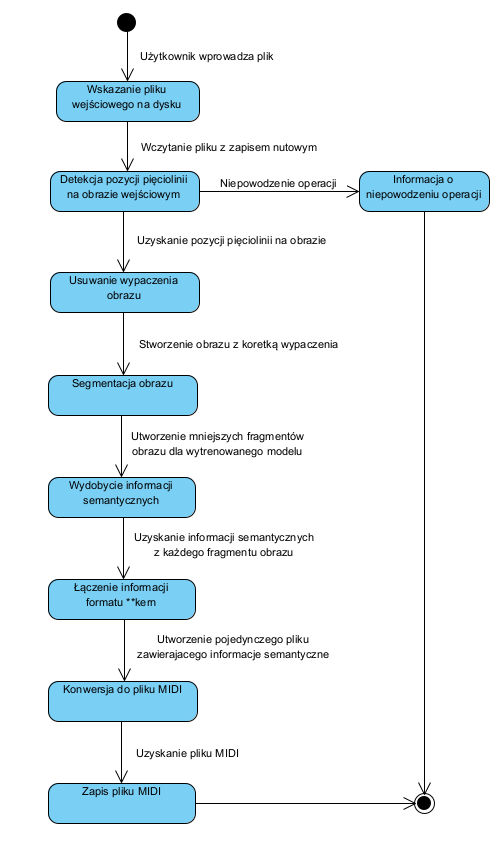
\includegraphics[width=10cm]{images/diagram-maszyny-stanowej-programu.png}
	\caption{Diagram maszyny stanowej programu.}
	\label{fig:program-state-machine}
\end{figure}


\section{Interfejs graficzny}

Interfejs został stworzony przy użyciu biblioteki \textit{PySimpleGUI}.

\begin{figure}[h]
	\centering
	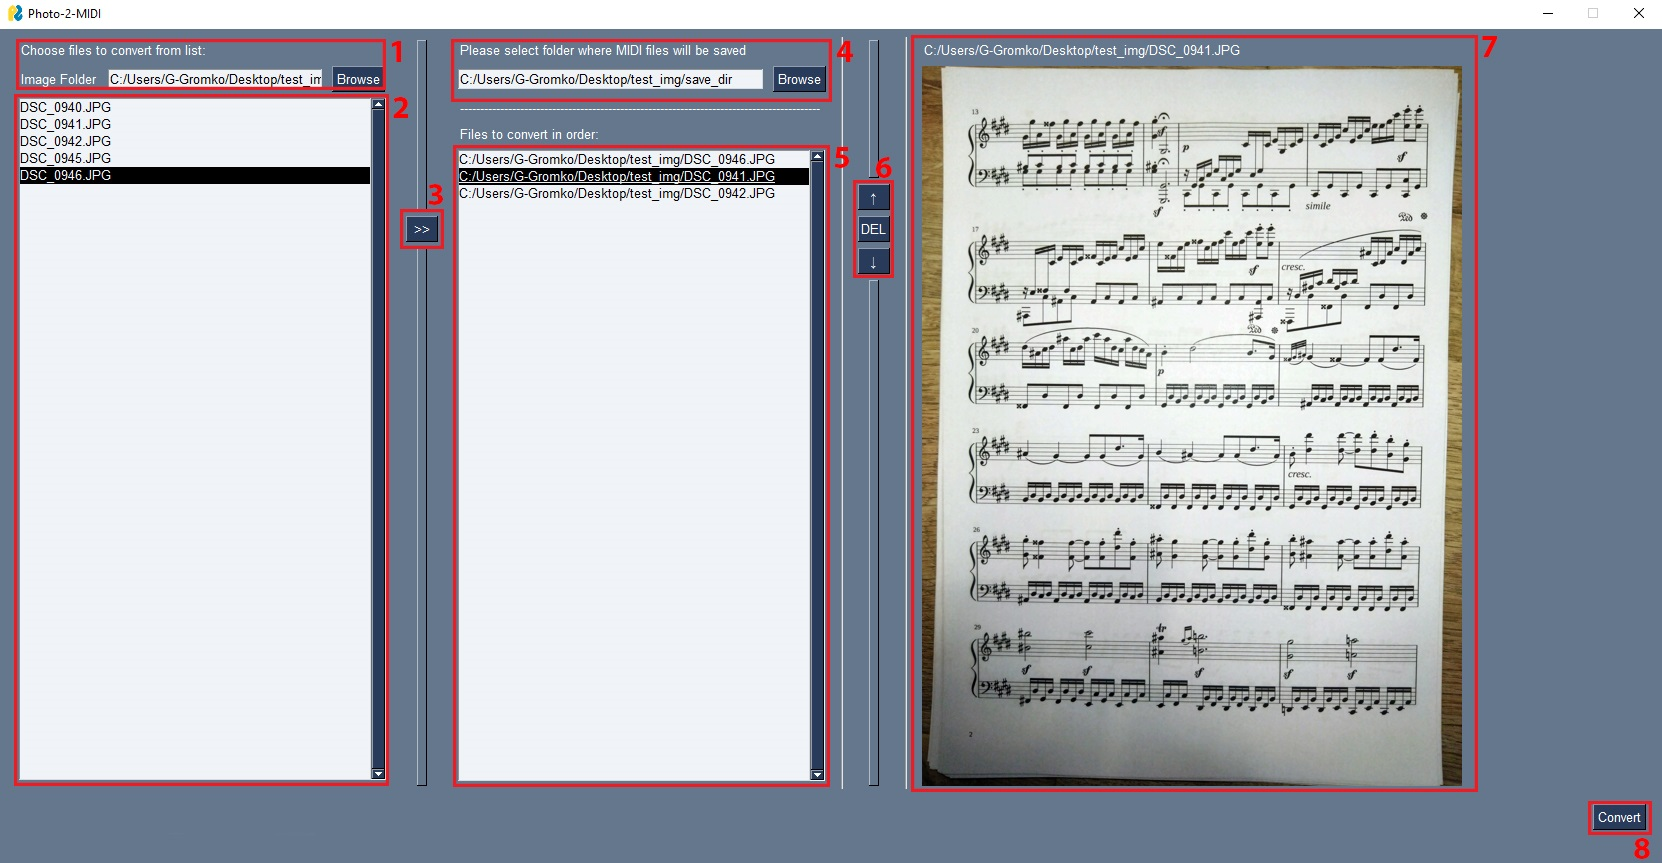
\includegraphics[width=16cm]{images/gui}
	\caption{Interfejs graficzny programu Photo-2-MIDI}
	\label{fig:gui}
\end{figure}

\begin{enumerate}
	\item Pole tekstowe do wprowadzenia ścieżki folderu ze zdjęciami zapisu nutowego.
	\item Lista plików w wybranym folderze.
	\item Przycisk do przeniesienia zaznaczonego pliku do listy plików do konwersji.
	\item Pole tekstowe do wprowadzenia ścieżki folderu do którego mają zostać zapisane uzyskane pliki MIDI.
	\item Lista plików przeznaczonym do konwersji, ułożone w kolejności w której konwersja ma się odbyć.
	\item Przyciski do organizacji plików przeznaczonych do konwersji, kolejno: przesuń wybrany plik w górę na liście, usuń wybrany plik z listy, przesuń wybrany plik w dół na liście.
	\item Podgląd wybranego pliku z jednej z list.
	\item Przycisk uruchamiający konwersję zdjęć do plików MIDI.
\end{enumerate}
\chapter{Użyte narzędzia programistyczne}
Rozdział ten zawiera opis narzędzi programistycznych wykorzystywanych podczas pracy nad projektem. 

\section{Git}
Jedno z najbardziej powszechnych i podstawowych narzędzi programistycznych, umożliwiające rozproszoną kontrolę wersji plików, która w przeciwieństwie do wielu alternatyw odbywa się lokalnie, gdyż każda kopia plików źródłowych kontrolowanych przez Gita może być pełnoprawnym repozytorium zawierającym całą historię zmian zachodzących na tychże plikach. Pozwala to na powrót do konkretnych wersji, których programista może potrzebować. Narzędzie to jest szeroko wykorzystywane do rozproszonego tworzenia oprogramowania przez grupy programistów w ramach jednego projektu, gdzie zmiany wprowadzane przez różnych ludzi są scalane do pojedynczego źródła, wykorzystując komercyjne rozwiązania hostowania online do przechowywania historii zmian.

Głównymi założeniami Gita jest:
\begin{itemize}
	\item Szybkość działania
	\item Elastyczność
	\item Bezpieczeństwo
	\item Wsparcie nielinowych, rozproszonych przepływów pracy
	\item Integralność danych
\end{itemize}

\section{Visual Studio Code}
Darmowy, otwartoźródłowy program do edycji, analizy i zarządzania kodem, stworzony i rozwijany przez Microsoft. Edytor ten jest z założenia edytorem minimalistycznym, zawierającym w swej podstawowej formie tylko niezbędne narzędzia, jednakże przez bycie projektem o otwartym źródle, jest on łatwo rozszerzalny dzięki szerokiej palecie wtyczek tworzonych przez podmioty komercyjne oraz członków społeczności. Szeroka gama rozszerzeń pozwala użytkownikom Visual Studio Code na dużą swobodę dostosowywania tego edytora pod swoje własne preferencje ergonomii pracy, jak i różnorodne projekty w większości języków programowania, przekształcając go w pełnoprawne interaktywne środowisko programistyczne, posiadające możliwość pracy ze zdalnymi zasobami.

Visual Studio Code posiada wbudowaną obsługę funkcji edycji kodu dla najpopularniejszych języków programowania takich jak:

\begin{itemize}
	\item Autouzupełnianie kodu
	\item Informacje dotyczące parametrów 
	\item Refactoring
	\item Analiza kodu
\end{itemize}
które to pozwalają na szybszą i bardziej efektywną pracę.
 

\section{Google Colaboratory}
Darmowa usługa chmurowa środowiska notatników Jupyter, pozwalająca na pisanie, wykonywanie i współdzielenie skryptów języka Python z poziomu przeglądarki internetowej. Główną zaletą tej usługi jest możliwość użytkowania zasobów zewnętrznego serwera, posiadającego znaczące moce obliczeniowe oraz wyspecjalizowany hardware do uczenia maszynowego, dając dostęp dla szerszej grupy ludzi do nauki i rozwoju w dziedzinie uczenia maszynowego i analizy danych, którzy nie mają dostępu do odpowiednich mocy obliczeniowych, wymaganych przez bardziej skomplikowane modele sztucznej inteligencji.
\chapter{Implementacja programu}
W rozdziale piątym zostały przedstawione najważniejsze fragmenty sposobu implementacji programu. 

\section{Realizacja detekcji pięciolinii}

Detekcja pięciolinii została opracowana na podstawie pracy M. Szwocha \textit{A Robust Detector for Distorted Music Staves}.

Jedną z najbardziej przydanych właściwości pięciolinii jest ich forma, mianowicie pięć prostych, równoodległych linii, co czyni je perfekcyjnymi kandydatami do detekcji zniekształceń wprowadzonych przez proces fotografowania, pozwalając na usunięcie niedoskonałości geometrycznych obrazu.

Proces detekcji pozycji pięciolinii na obrazie został zrealizowany przy pomocy analizy histogramów okienek próbnikowych. Okienkiem próbnikowym nazywany jest fragment obrazu rozciągający się na całą jego wysokość i pewną szerokość, przy pomocy którego dokonywana jest analiza obrazu, poprzez analizę jego mniejszych fragmentów. Po analizie okienka na danej części obrazu, jego pozycja jest przesuwana o daną odległość w osi poziomej, po czym następuje analiza następnego wycinka. Poszczególne okienka próbnikowe nie mają na siebie bezpośredniego wpływu podczas analizy.

\begin{figure}[H]
	\centering
	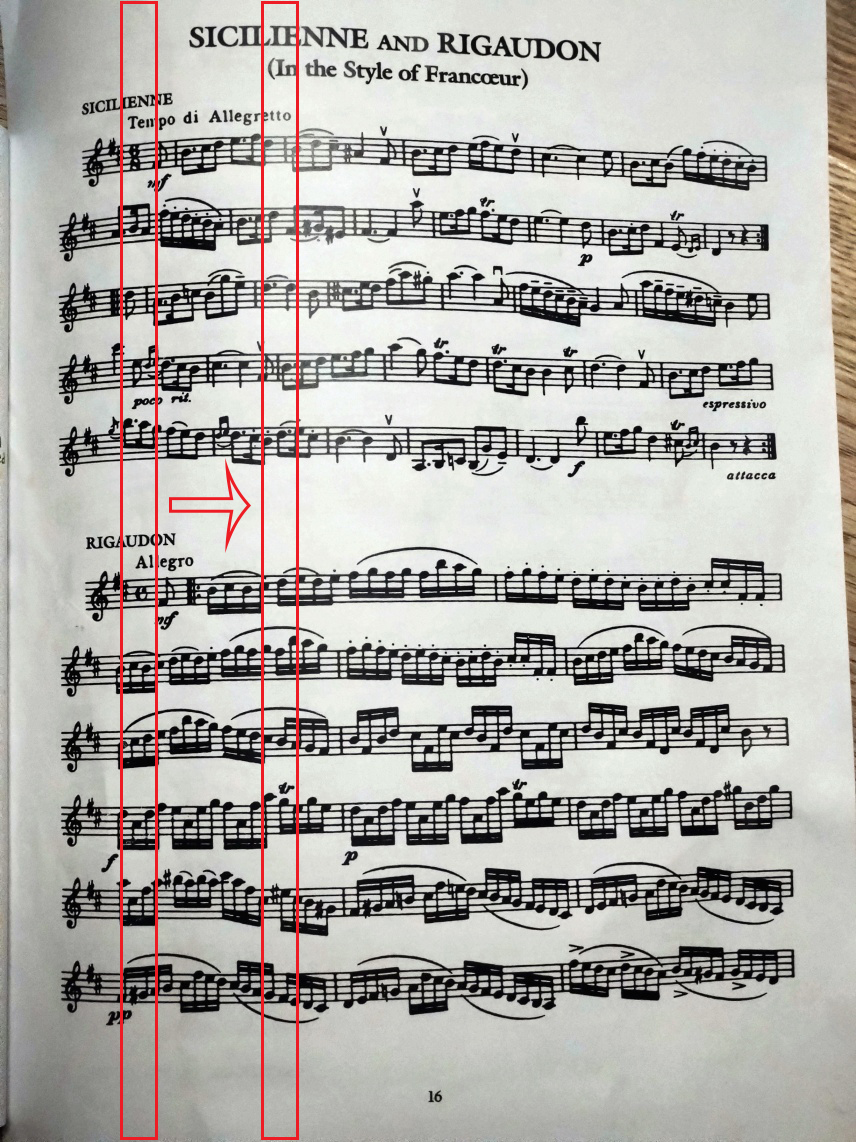
\includegraphics[width=12cm]{images/probe window demo.jpg}
	\caption{Wizualizacja okienka próbnikowego na zdjęciu nut.}
	\label{fig:probe_window_demo}
\end{figure}

\pagebreak

\subsection{Realizacja detekcji pozycji wypaczonych pięciolinii na obrazie}

\begin{lstlisting}[caption={\pyth|find_staves_points()| - funkcja odnajdywania pozycji pięciolinii na obrazie}, label={find-staves-points}, language=Python]
def find_staves_points(img, img_name, stride = 2):
	img = enhance_image(img, img_name)
	
	img_y, img_x = img.shape[:2]
	
	staff_line_dist = find_staff_line_distance(img)
	if staff_line_dist == -1:
		return -1, 0
	
	staves_positions = find_staves_positions(staff_line_dist, stride, img)
	if len(staves_positions) == 0:
		return -1, -1
	else:
		staves_points_list = make_staves_points_list(staves_positions, staff_line_dist)
		if staves_points_list == -1  or len(staves_points_list) == 0:
			return -1, -1

	return staves_points_list, staff_line_dist
\end{lstlisting}

Powyższa funkcja \pyth|texfind_staves_points()| jest odpowiedzialna za znalezienie i stworzenie listy punktów, które definiują pozycję pięciolinii. Funkcja ta przyjmuje za argumenty wczytany obraz, jego nazwę oraz liczbę kroków. Natomiast zwraca listę zawierającą punkty opisujące położenie pięciolinii oraz odległość między liniami pięciolinii, albo wartości zawiadamiające kod wywołujący tę funkcję o wystąpieniu błędu.

Pierwszym krokiem do poprawnej detekcji pięciolinii na obrazie jest uwydatnienie pożądanych jego cech, co jest wykonywane przy pomocy funkcji \pyth|enchance_image()|, dzięki której możliwa jest łatwiejsza analiza badanego obrazu. Następnie następuje wywołanie funkcji odpowiedzialnej za odnalezienie odległości pomiędzy liniami pięciolinii \pyth|find_staff_line_distance()|, poprzez przekazanie obrazu. Jeśli tejże funkcji udało się poprawie odnaleźć szukaną wartość, następuje wywołanie kodu mającego odszukać pozycje pięciolinii na obrazie \pyth|find_staves_positions()| przez przekazanie odnalezionej wcześniej odległości, liczby kroków oraz obrazu. Kiedy operacja się powiedzie, następuje reformatowanie listy uzyskanych punktów przez funkcję \pyth|make_staves_points_list()|, by punkty zawarte w jednej liście zawierały pozycje pojedynczej pięciolinii. Operacja ta jest potrzebna, gdyż uzyskane wartości są ułożone w listach reprezentujących pozycje w pionowych wycinkach, gdzie następna część programu będzie potrzebowała ich w formacie punktów pojedynczej pięciolinii na jedna listę. W wypadku powodzenia wszystkich operacji następuje zwrot listy pozycji oraz odległości pomiędzy liniami pięciolinii.



\subsubsection{Realizacja uwydatniania obrazu} \label{enhance_image_impl}

\begin{lstlisting} [caption={\pyth|enhance_image()| - funkcja uwydatniania obrazu.}, label={enhance-image}, language=Python]
	def enhance_image(img):
	if len(img.shape) == 3:
		img = cv2.cvtColor(img, cv2.COLOR_RGB2GRAY)
	
	img = cv2.GaussianBlur(img, (5, 5), 0)
	img = cv2.adaptiveThreshold(img, 255, cv2.ADAPTIVE_THRESH_MEAN_C, cv2.THRESH_BINARY, 55, 7)
	
	return img
\end{lstlisting}

Znajdująca się powyżej funkcja ma za zadanie zmodyfikowanie obrazu, by ten nadawał się do jego analizy. Odbywa się to przez konwersję obrazu do odcieni szarości, jeśli jest on obrazem kolorowym, po czym następuje seria modyfikacji, pozwalających na uwydatnienie pożądanych informacji z obrazu.

Pierwszą modyfikacją jest rozmycie gaussowskie, dzięki któremu z obrazu usuwana jest część szumu oraz drobne niedoskonałości są rozmywane, by w następnym kroku możliwe było lepsze określenie wartości znajdujących się ponad progiem. Kolejną modyfikacją zastosowaną na obrazie jest progowanie adaptacyjne, które w przeciwieństwie do zwykłego progowania, pozwala na usunięcie cieni z obrazu, zachowując znajdujące się w nich dane, które mogą być potrzebne do poprawnej analizy. Jednocześnie progowanie adaptacyjne automatycznie znajduje odpowiednie wartości progu, dzięki czemu nie istnieje potrzeba określania go ręcznie, co wymaga znaczącej ilości czasu i prób, by znaleźć taką wartość, która będzie działała w jak najszerszym zakresie danych wejściowych. Ostatnią modyfikacją dotykającą obraz jest erozja, która służy do usunięcia niechcianych punktów i wyostrzenie linii znajdujących się na obrazie, co jest wymagane dla poprawnego odszukiwania pięciolinii.



\subsubsection{Realizacja odnajdywania odległości między liniami pięciolinii} \label{find_staff_line_distance_impl}

\begin{lstlisting} [caption={ \pyth|find_staff_line_distance()| - funkcja odnajdywania odległości między liniami pięciolinii.}, label={find-staff-line-distance}, language=Python]
def find_staff_line_distance(img = np.array):
	img_y, img_x = img.shape[:2]
	probe_window_size = img_x // 40
	probe_window_start_idx = img_x // 5
	probe_window_end_idx = img_x - probe_window_start_idx
	probe_window_hist_arr = np.zeros(img_y)
	staff_line_distance_list = []
	
	for i in range(probe_window_start_idx, probe_window_end_idx, probe_window_size*6):
		make_histogram_array(i, img_y, probe_window_size, img, probe_window_hist_arr)
		peaks_list = filter_out_peaks(probe_window_size, probe_window_hist_arr)
		staff_line_distance = find_staff_line_distance_in_probe(peaks_list)
		
		if staff_line_distance != 0:
			staff_line_distance_list.append(staff_line_distance)
		
		probe_window_hist_arr = np.zeros(img_y)
	
	if len(staff_line_distance_list) != 0:
		return sum(staff_line_distance_list) // len(staff_line_distance_list)
	else:
		return -1
\end{lstlisting}

Umieszczony powyżej kod funkcji \pyth|find_staff_line_distance()| odpowiedzialny jest za odnalezienie odległości pomiędzy liniami pięciolinii na zdjęciu zapisu nutowego. Funkcja ta zaczyna pracę poprzez inicjalizację niezbędnych zmiennych zawierających wartości takie jak: rozmiary obrazu, rozmiar okienka próbnikowego, indeks początkowy poszukiwania, indeks końcowy, tablicę na której będą przechowywane wartości odczytane z okienka próbnikowego, oraz lista potencjalnych odległości z okienek próbnikowych.

Wartości tych zmiennych nie są przypadkowe, szerokość okienka została dobrana eksperymentalnie, podczas to których eksperymentów stwierdzono, iż wielkość równa jednej czterdziestej szerokości obrazu daje zadowalające rezultaty, dające poprawne wielkości, natomiast pozycja początkowa i końcowa okienka próbnikowego gwarantuje, na poprawnie wykonanych zdjęciach, znajdowanie się pięciolinii w badanym zakresie.

Właściwe odszukiwanie odbywa się iteratywnie poprzez przesuwanie okienka próbnikowego o wielkości większe od jego szerokości, gdyż nie potrzebujemy analizować całego obrazu, tylko kilka jego fragmentów. Analizowanie pojedynczego okienka może dać niepoprawną wartość odległości, zatem obraz jest analizowany w kilku miejscach, by pozyskać właściwą miarę.

W każdym kroku pętli tworzona jest tablica, na podstawie której powstaje histogram okienka, dzięki funkcji \pyth|make_histogram_array()|, która zlicza wystąpienia ciemnych pikseli w  każdym rzędzie badanego okienka. Następnie z uzyskanej tablicy, w funkcji \pyth|filter_out_peaks|, odfiltrowywane są indeksy wysokich wartości histogramu, które powinny być liniami rozpinającymi się na większość szerokości okienka. Na podstawie uzyskanej listy indeksów w funkcji \pyth|find_staff_line_distance()| odszukiwana jest odległość między liniami pięciolinii, dzięki własności zapisu nutowego, w którym najczęściej występującą odległością między dwiema liniami w osi pionowej jest właśnie odległość pomiędzy składowymi pięciolinii. Jeśli odnaleziona wartość nie jest zerem, to jest dodawana do listy potencjalnych odległości. Przed przejściem do następnego kroku pętli, tablica okienka próbnikowego jest zerowana, by poprzednia analiza nie wpływała na analizę kolejnego okienka.

Gdy analiza okienek się zakończy, jeśli lista potencjalnych odległości nie jest pusta, zwracana jest średnia arytmetyczna z listy odległości w formie wartości całkowitej, natomiast jeśli lista jest pusta, zwracana jest wartość \textit{-1}, by poinformować kod wywołujący o błędzie operacji.



\subsubsection{Realizacja odnajdywania pozycji pięciolinii}

\begin{lstlisting}[caption={\pyth|find_staves_positions()| - funkcja odnajdywania pozycji pięciolinii.}, label={find-staves-positions}, language=Python]
def find_staves_positions(staff_line_distance, stride = 1, img = np.array):
	img_y, img_x = img.shape[:2]
	probe_window_size = (staff_line_distance * 2) + 5
	probe_window_start_idx = probe_window_size * 2
	probe_window_end_idx = img_x - probe_window_start_idx
	probe_window_hist_arr = np.zeros(img_y)
	staves_positions_list = []
	
	for i in range(probe_window_start_idx, probe_window_end_idx, probe_window_size * stride):
		make_histogram_array(i, img_y, probe_window_size, img, probe_window_hist_arr)
		peaks_list = filter_out_peaks(probe_window_size, probe_window_hist_arr)
		staves_positions = get_staves_positions(i, staff_line_distance, peaks_list)
		staves_positions_list.append(staves_positions)
		
		probe_window_hist_arr = np.zeros(img_y)
	
	if len(staves_positions_list) == 0:
		return -1
	else:
		return staves_positions_list
\end{lstlisting}

Odszukiwanie pozycji pięciolinii, realizowane w funkcji \pyth|find_staves_positions()| odbywa się analogicznie do działania \pyth|find_staff_line_distance|, z pewnymi różnicami, mianowicie:
\begin{itemize}
	\item szerokość okienka próbnikowego wynosi dwukrotność odległości między liniami pięciolinii, plus pięć pikseli. Wynika to z właściwości zapisu nutowego, gdzie główka nuty jest nieco szersza, niż odległość między liniami, przez co taka wartość zapewnia, że główka nuty nie będzie zajmowała całej szerokości badanej części obrazu, zaburzając odczytywane dane, scalając ze sobą dwie linie.
	\item początkowa pozycja jest ustalona na dwie szerokości okienka od lewej krawędzi, końcowa zaś na dwie szerokości od prawej krawędzi, by uniknąć niepotrzebnej analizy granic obrazu, na których zazwyczaj nic się nie znajduje, lub znajdują się tam losowe wartości uzyskane z tła.
	\item szerokość kroku jest uzależniona od szerokości okienka oraz przekazanej wartości kroku, która mówi o ile okienko ma się przesuwać w każdym kroku pętli.
	\item po odnalezieniu indeksów dużych wartości histogramu w każdym korku pętli, wywoływana jest funkcja \pyth|get_staves_postitions|, która szuka sekwencji, odległych od siebie o wcześniej odszukaną odległość pięciu indeksów na całej wysokości okienka, tworząc listę punktów z danego wycinka, na którym znajdują się pięciolinie. Zwrócona lista jest dodawana do listy pozycji na których zostały wykryte pięciolinie, po czym resetowana jest tablica okienka próbnikowego.
\end{itemize}


Gdy analiza okienek się zakończy, jeśli lista pozycji nie jest pusta, to jest ona zwracana, natomiast jeśli lista jest pusta, zwraca się wartość \textit{-1}, by poinformować kod wywołujący o błędzie operacji.

\section{Usuwanie wypaczania obrazu}

\section{Segmentacja obrazu}

\section{Model głębokiego uczenia do rozpoznawania zapisu nutowego}



\summary
Tu podsumowanie z realizacji założeń, możliwości dalszej pracy

\bibliographystyle{plain}
\bibliography{literatura}

% spis tabel
\listoftables

% spis rysunków
\listoffigures

% spis listingów
\lstlistoflistings

\end{document}
